\chapter{Bäume}

\begin{itemize}
  \item Verallg. von Listen: Element/Knoten kann mehrere Nachfolger haben
  \item Darstellung von Hierarchien
\end{itemize}

\paragraph{Ungerichteter Graph}
\index{Ungerichteter Graph}
$(V, E)$ mit einer Menge Knoten $V$ und Kanten $E \subseteq V \times V$

\paragraph{Baum}
\index{Baum}
Ungerichteter Graph mit

\begin{mzImportant}
  \begin{description}
    \item [Einfach] keine Schleife
          \mzInline{
            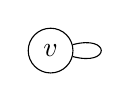
\begin{tikzpicture}[every loop/.style={}]
              \node [circle,draw] {$v$} edge[loop right] ();
            \end{tikzpicture}
          }
          oder Doppelkanten
          \mzInline{
            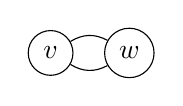
\begin{tikzpicture}
              \node (v) [circle,draw] {$v$};
              \node (w) at (1,0) [circle,draw] {$w$};
              \path (v) edge [bend left] (w);
              \path (w) edge [bend left] (v);
            \end{tikzpicture}
          }
          \index{Einfacher Graph}

    \item [Zusammenhängend]
          \index{Zusammenhängender Graph}
          Für jede zwei Knoten gibt es genau eine Folge von Kanten die sie verbindet

    \item [Azyklisch]
          \index{Azyklischer Graph}
          kein Zyklus (Cycle)
          \mzInline{
            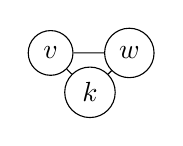
\begin{tikzpicture}
              \node (v) [circle,draw] {$v$};
              \node (w) at (1,0) [circle,draw] {$w$};
              \node (k) at (.5,-.5) [circle,draw] {$k$};

              \draw (v) -- (w) -- (k) -- (v);
            \end{tikzpicture}
          }
  \end{description}
\end{mzImportant}

\paragraph{Wurzelbaum}
\index{Wurzelbaum}
Baum mit genau einem Knoten der Wurzel hei\ss t

\paragraph{Orientierter Wurzelbaum}
\index{Orientierter Wurzelbaum}
Alle Knoten sind Wurzel ihrer disjunkten Unterbäume und haben verschiedene Werte gleichen Typs. (Im Nachfolgenden einfach nur ,,Baum``)

% TODO: TikZ Grafik für Wurzelbaumterminologie

\paragraph{Darstellungsarten}

% TODO: TikZ Grafiken
\begin{description}
  \item[Graph]
    \mzInline{
      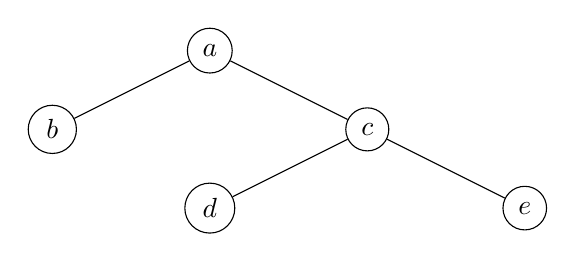
\begin{tikzpicture}[xscale=2]
        \node (b) at (0,0) [circle,draw] {$b$};
        \node (a) at (1,1) [circle,draw] {$a$};
        \node (c) at (2,0) [circle,draw] {$c$};
        \node (d) at (1,-1) [circle,draw] {$d$};
        \node (e) at (3,-1) [circle,draw] {$e$};

        \draw (b) -- (a) -- (c) -- (e);
        \draw (c) -- (d);
      \end{tikzpicture}
    }
    \mzInline{
      \begin{tikzpicture}[xscale=2]
        \node (b) at (0,0) [circle,draw] {$b$};
        \node (a) at (1,1) [circle,draw] {$a$};
        \node (c) at (2,0) [isosceles triangle,shape border rotate=90,draw] {$T_r$};

        \draw (b) -- (a) -- (c.apex);
      \end{tikzpicture}
    }
  \item[Array] $[a,b,c,\emptyset,\emptyset,d,e]$
    % \item[Verkettete Liste]
    % \item[Einrückung]
  \item[Menge] $\{\{a,b,c,d,e\},\{b\},\{c,d,e\},\{d\},\{e\}\}$
  \item[Klammer] $(a, (b), (c, (d), (e)))$
\end{description}

\paragraph{Grö\ss en}

\begin{mzImportant}
  \begin{description}
    \item[Ordnung] Max. Anzahl von Kindern jedes Knoten eines Baums
      \index{Baumordnung}

    \item[Tiefe] Anzahl Kanten zwischen einem Knoten und Wurzel
      \index{Knotentiefe}

    \item[Stufe] Alle Knoten gleicher Tiefe
      \index{Baumstufe}

    \item[Höhe] Max. Tiefe $+ 1$
      \index{Baumhöhe}
  \end{description}
\end{mzImportant}

\paragraph{Eigenschaften}

\begin{mzImportant}
  \begin{description}
    \item[Geordnet] Kinder erfüllen Ordnung von links nach rechts
      \index{Geordneter Baum}

    \item[Vollständig]
      \index{Vollständiger Baum}
      Alle Blätter auf gleicher Stufe, jede Stufe hat max. Anzahl von Kindern
  \end{description}
\end{mzImportant}

\section{Binärbäume}
\index{Binärbaum}

Geordneter, orientierter Wurzelbaum der Ordnung $2$.

\begin{mzImportant}
  \begin{description}
    \item[Strikt]
      \index{Strikter Binärbaum}
      Jeder Knoten hat $0$ oder $2$ Kinder (Kein Knoten hat genau $1$ Kind).

    \item[Vollständig]
      \index{Vollständiger Binärbaum}
      Jeder Knoten au\ss er der letzten Stufe hat genau $2$ Kinder.

    \item[Fast Vollständig]
      \index{Fast Vollständiger Binärbaum}
      Vollständig, außer Blätter können rechts fehlen.

    \item[Ausgeglichen]
      \index{Ausgeglichener Binärbaum}
      Vollständig, aber Blätter auf letzten $2$ Stufen
  \end{description}
\end{mzImportant}

$2$ Binärbäume hei\ss en

\begin{description}
  \item[Ähnlich] selbe Struktur
    \index{Ähnliche Binärbäume}

  \item[Äquivalent] Ähnlich und selbe Knoten
    \index{Äquivalte Binärbäume}
\end{description}

\paragraph{Grö\ss en}

\begin{itemize}
  \item Für $i$ Stufen max. $2^i$ Knoten
  \item Für $n$ Knoten genau $n - 1$ Kanten
  \item Vollständiger B. mit $n$ Knoten hat Höhe von $\log_2 n + 1$
\end{itemize}

\subsection{Speicherung}
\index{Speicherung von Binärbäumen}

\begin{description}
  \item[Verkettet] \fbox{Zeiger Links | Knoten | Zeiger Rechts}
  \item[Feldbaum] Sequenz von \fbox{Knoten | Index Links | Index Rechts}
  \item[Sequenziell] Lesen vollst. Baum links nach rechts, oben nach unten, leere Elemente für fehlende Knoten (ineffizient für degenerierte Bäume)
\end{description}

\subsection{Traversierung}
\index{Traversierung}

\begin{itemize}
  \item $W$ Verarbeite Wurzel
  \item $L$ Durchlaufe linken Unterbaum
  \item $R$ Durchlaufe rechten Unterbaum
\end{itemize}

Konvention erst links, dann rechts:

\begin{itemize}
  \item $WLR$ Preorder
        \index{Preorder}
        \index{Vorordnung}
  \item $LWR$ Inorder
        \index{Inorder}
        \index{Zwischenordnung}
  \item $LRW$ Postorder
        \index{Postorder}
        \index{Nachordnung}
\end{itemize}

Implementation rekursiv oder linear mit eigenem Stack (effizienter)

\subsection{Gefädelte Binärbäume}
\index{Gefädelter Binärbaum}

Zeiger ,,Faden`` in Knoten zeigt auf nächsten Knoten nach Durchlaufordnung.

Nachteil: Zusätzlicher Speicheraufwand teilweise redundant; Lösung: Nur Null-Zeiger (Blätter) sind Fäden

\begin{description}
  \item[rFaden] zeigt auf Nachfolgerknoten
    \index{rFaden}
  \item[lFaden] zeigt auf Vorgängerknoten
    \index{lFaden}
\end{description}

\section{Binäre Suchbäume}
\index{Binärer Suchbaum}

\subsection{Natürliche binäre Suchbäume}
\index{Natürlicher Binärer Suchbaum}

$$B_l < B_x < B_r$$

\begin{description}
  \item [Suchen] rekursiv oder mit Durchlaufalg. $\in O(\ln n)$
  \item [Einfügen] dort wo Suche terminiert
  \item [Löschen] mit zwei nicht-leeren Unterbäumen: Hochziehen des grö\ss ten Wertes im linken oder kleinsten Wert im rechten Unterbaum (Alt: Als gelöscht markieren)
\end{description}

\subsection{Balancierte Binärbäume}
\index{Blancierter Binärbaum}

Grundoperationen auf ausgeglichene Binärbäume kosten am wenigsten. Herstellung der Ausgeglichenheit in $O(n)$

\begin{description}
  \item [Balancefaktor] von Knoten $x$ ist $BF(x) := h(B_l (x)) - h(B_r (x))$
        \index{Balancefaktor}

  \item[$k$-Balanciert] $\forall x \in B: |BF(x)| \leq k$
    \index{k-Balanciert}
\end{description}

\paragraph{AVL-Baum} 1-balancierter Binärer Suchbaum
\index{AVL-Baum}

Herstellung der Ausgeglichenheit durch Rotationen
\index{Rotationen auf AVL-Bäumen}

% TODO: TikZ Grafik

\begin{itemize}
  \item $BF(u) = -2, BF(v) \in \{ 0, -1 \}$: Einfachrotation $\mathbf{\text{Links}(u)}$
  \item $BF(u) = +2, BF(v) \in \{ 0, -1 \}$: Einfachrotation $\mathbf{\text{Rechts}(u)}$
  \item $BF(u) = -2, BF(v) = +1$: Doppelrotation $\mathbf{\text{Rechts}(v) + \text{Links}(u)}$
  \item $BF(u) = +2, BF(v) = -1$: Doppelrotation $\mathbf{\text{Links}(v) + \text{Rechts}(u)}$
\end{itemize}

Für jeden AVL-Baum $T$ der Höhe $h$ gilt:

\begin{itemize}
  \item $|T| \geq F_h$ (Fibonacci)
  \item $h \leq \frac{\log_2 (n\sqrt{5} + 1)}{\log_2 (\frac{1 + \sqrt{5}}{2})}$
\end{itemize}

\paragraph{Fibonacci-Bäume}
\index{Fibonacci-Baum}

$B_0$ ist leerer Baum, $B_1$ ist einzelner Knoten, $B_h = \texttt{BUILD}(B_{h-1}, x, B_{h-2})$ für $h \geq 2$

(Maximal unbalancierter AVL-Baum der Höhe h)

\subsection{Gewichtsbalancierte Binärbäume}
\index{Gewichtsbalancierter Binärbaum}

\begin{description}
  \item[Wurzelbalance]
    \index{Wurzelbalance}
    $\rho (B) = \frac{n_l + 1}{n + 1}$ mit $n$ Knoten und $n_l$ Knoten im linken Unterbaum

  \item [Gewichtsbalanciert (BB)] $\forall \text{ Unterbaum } B': \alpha \leq \rho(B') \leq 1 - \alpha$

        \begin{itemize}
          \item $\alpha = 1/2$: Vollst. Binärbaum
          \item $\alpha < 1/2$: Zunehmend weniger ausgeglichen
          \item $\alpha = 0$: Keine Einschränkung
        \end{itemize}
\end{description}

% \subsection{Positionssuche in balancierten Bäumen}

